\section{Heat Exchange Through Ground Loop}
To isolate the ground loop for further studying we will first look at what type energy is needed and expected from the ground loop to dissipate. In this case we will consider a average four bedroom home heat lost. This would normally be calculated using the Manual J. form provided by the ACCA \cite{ACCAManualJ}, but here we will focus on a hypothetical scenario. It is important for contractors to properly calculate the heat lost estimates. The Manual J. provides the designer with a room by room energy lost and a whole house energy lost. Using this information any heating or cooling system can be properly sized. Since we are focusing on a hypothetical case, we can create constraints that will allow us to look at specific individual parts of the system. \\ \\
%
We will consider the geo-thermal heat pump ground loop. This is the main component that has a large about of variations based on the different environments and soil conditions offered. All cooling loop designs aim to cool down the working fluid by transferring heat to the outside medium. The most common is to bury the cooling loops in the ground, but another option is to put the loops in a larger body of water such as a pond or lake. Within the soil, cooling loops have many different type of configurations. To explain these visually, please examine the figures below.
%
\begin{figure}[H]
    \centering
    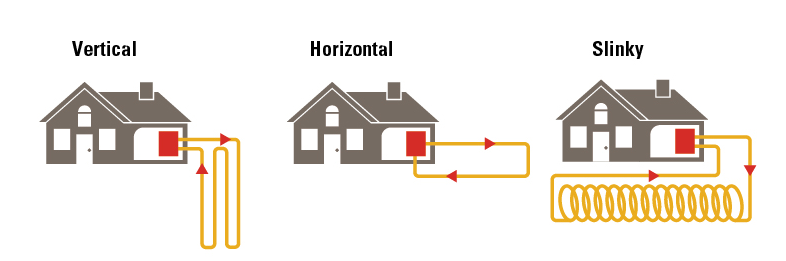
\includegraphics[width=6in]{pictures/GroundLoops.png}
    \caption{Different closed loop geothermal cooling loops. \textit{Mississippi Power \cite{GCHP}}}
\end{figure}
%
\noindent
One of the common types of configurations is the vertical well. Vertical holes are drilled several meters into the ground and a u-shaped pipe is put vertically into the column. This vertical method is popular because the yard of the customer's house does not need to be torn up, and because it reaches deeper into the constant temperature soil it is less effected by the above ground weather. With each of these types they come in two configurations series and parallel. In the next section we will formulate the problem and look at the heat transfer between the ground loop and the outside soil.